\section{Maximum Three-Way Conference Rooms Tests}
\label{sec:conf-rooms-test}

The conference rooms test was developed primarily for executing three-way conferences.
Basically, there is a conference with three participants started. After that, there is another conference
with three participants started until the maximum number of conferences is reached:

\begin{figure} [!ht]
\centering
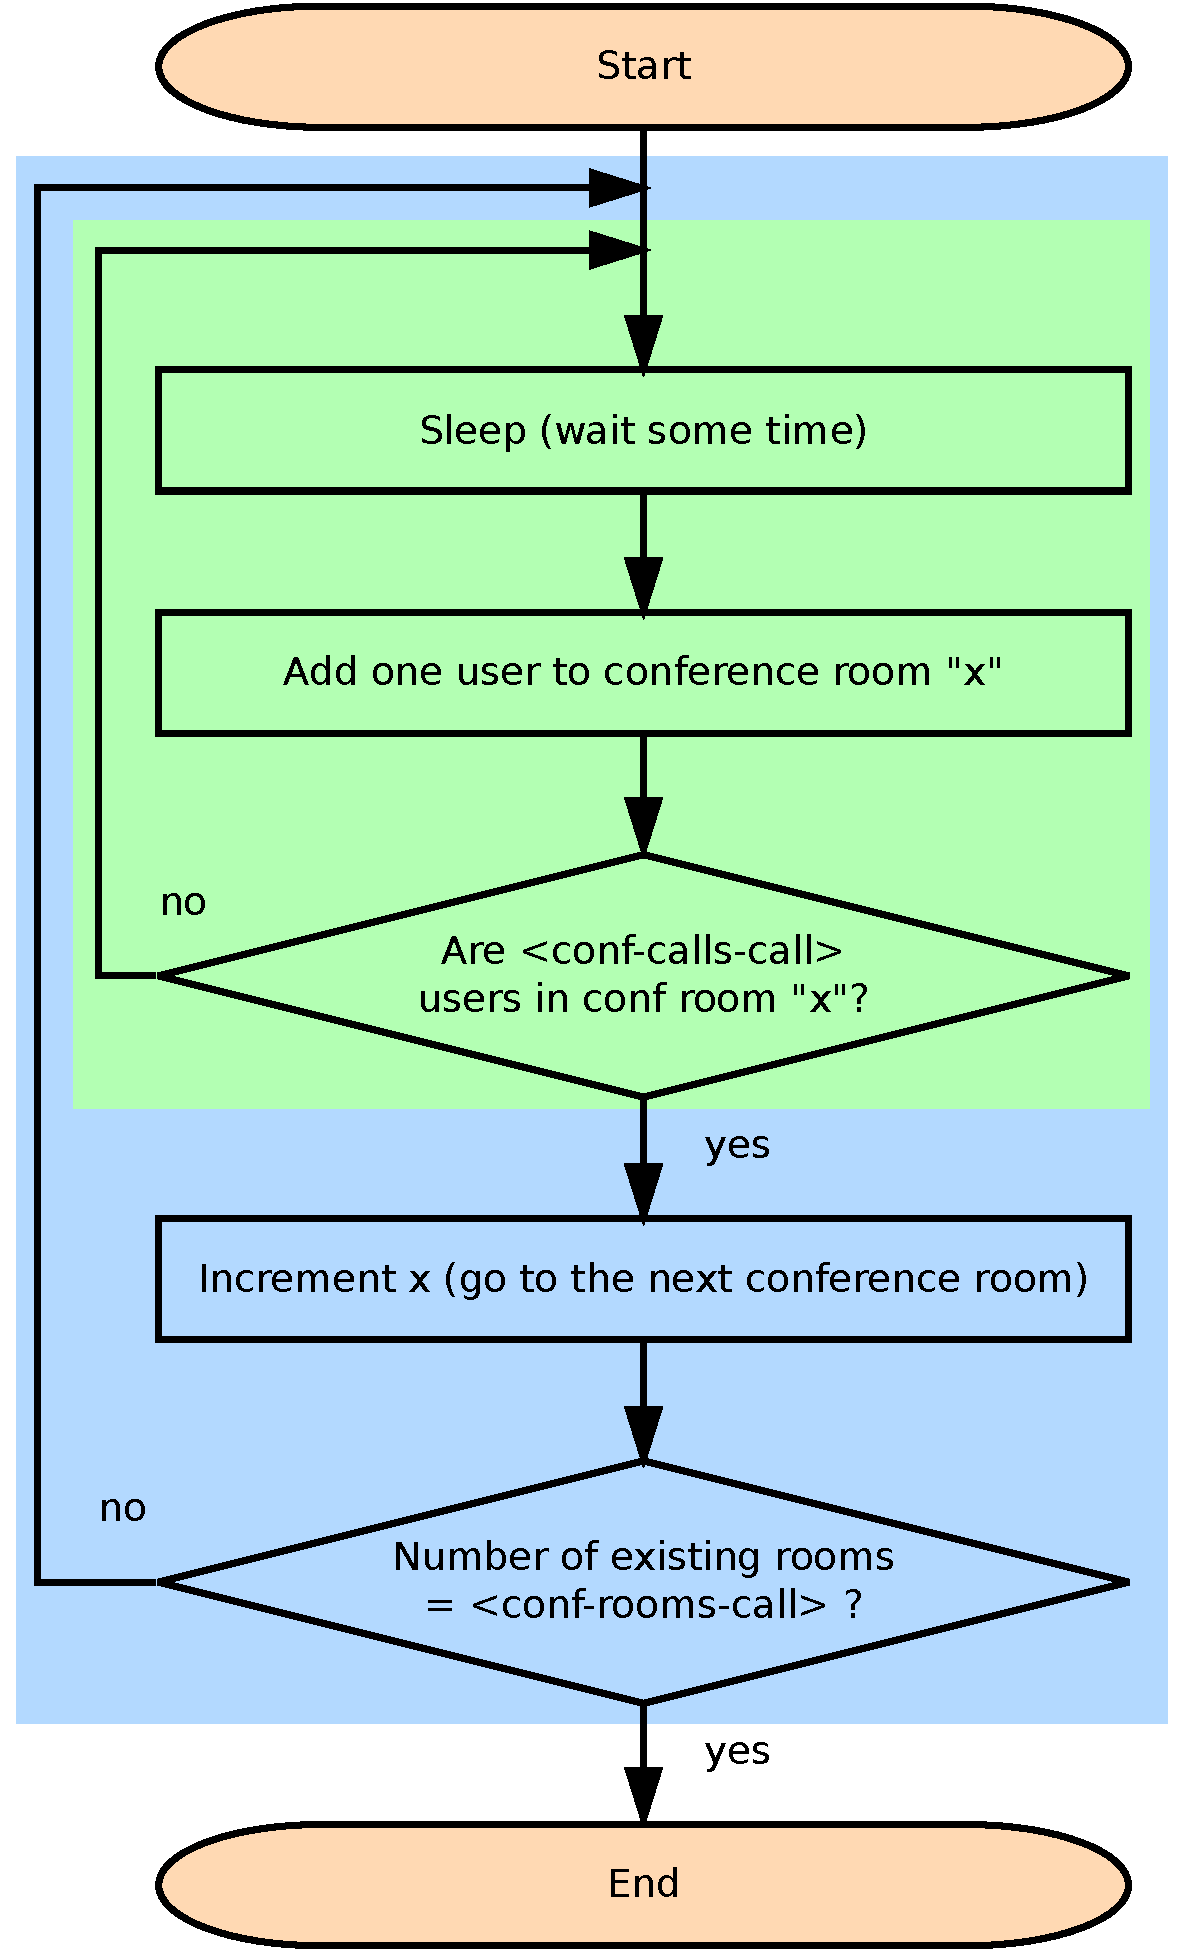
\includegraphics [width=8cm] {conf-rooms-test-1}
\caption{Process of conference rooms tests}
\end{figure}

For a conf call test with three participants and four conference rooms, the test would work like this: \newpage
\begin{figure} [!ht]
\centering
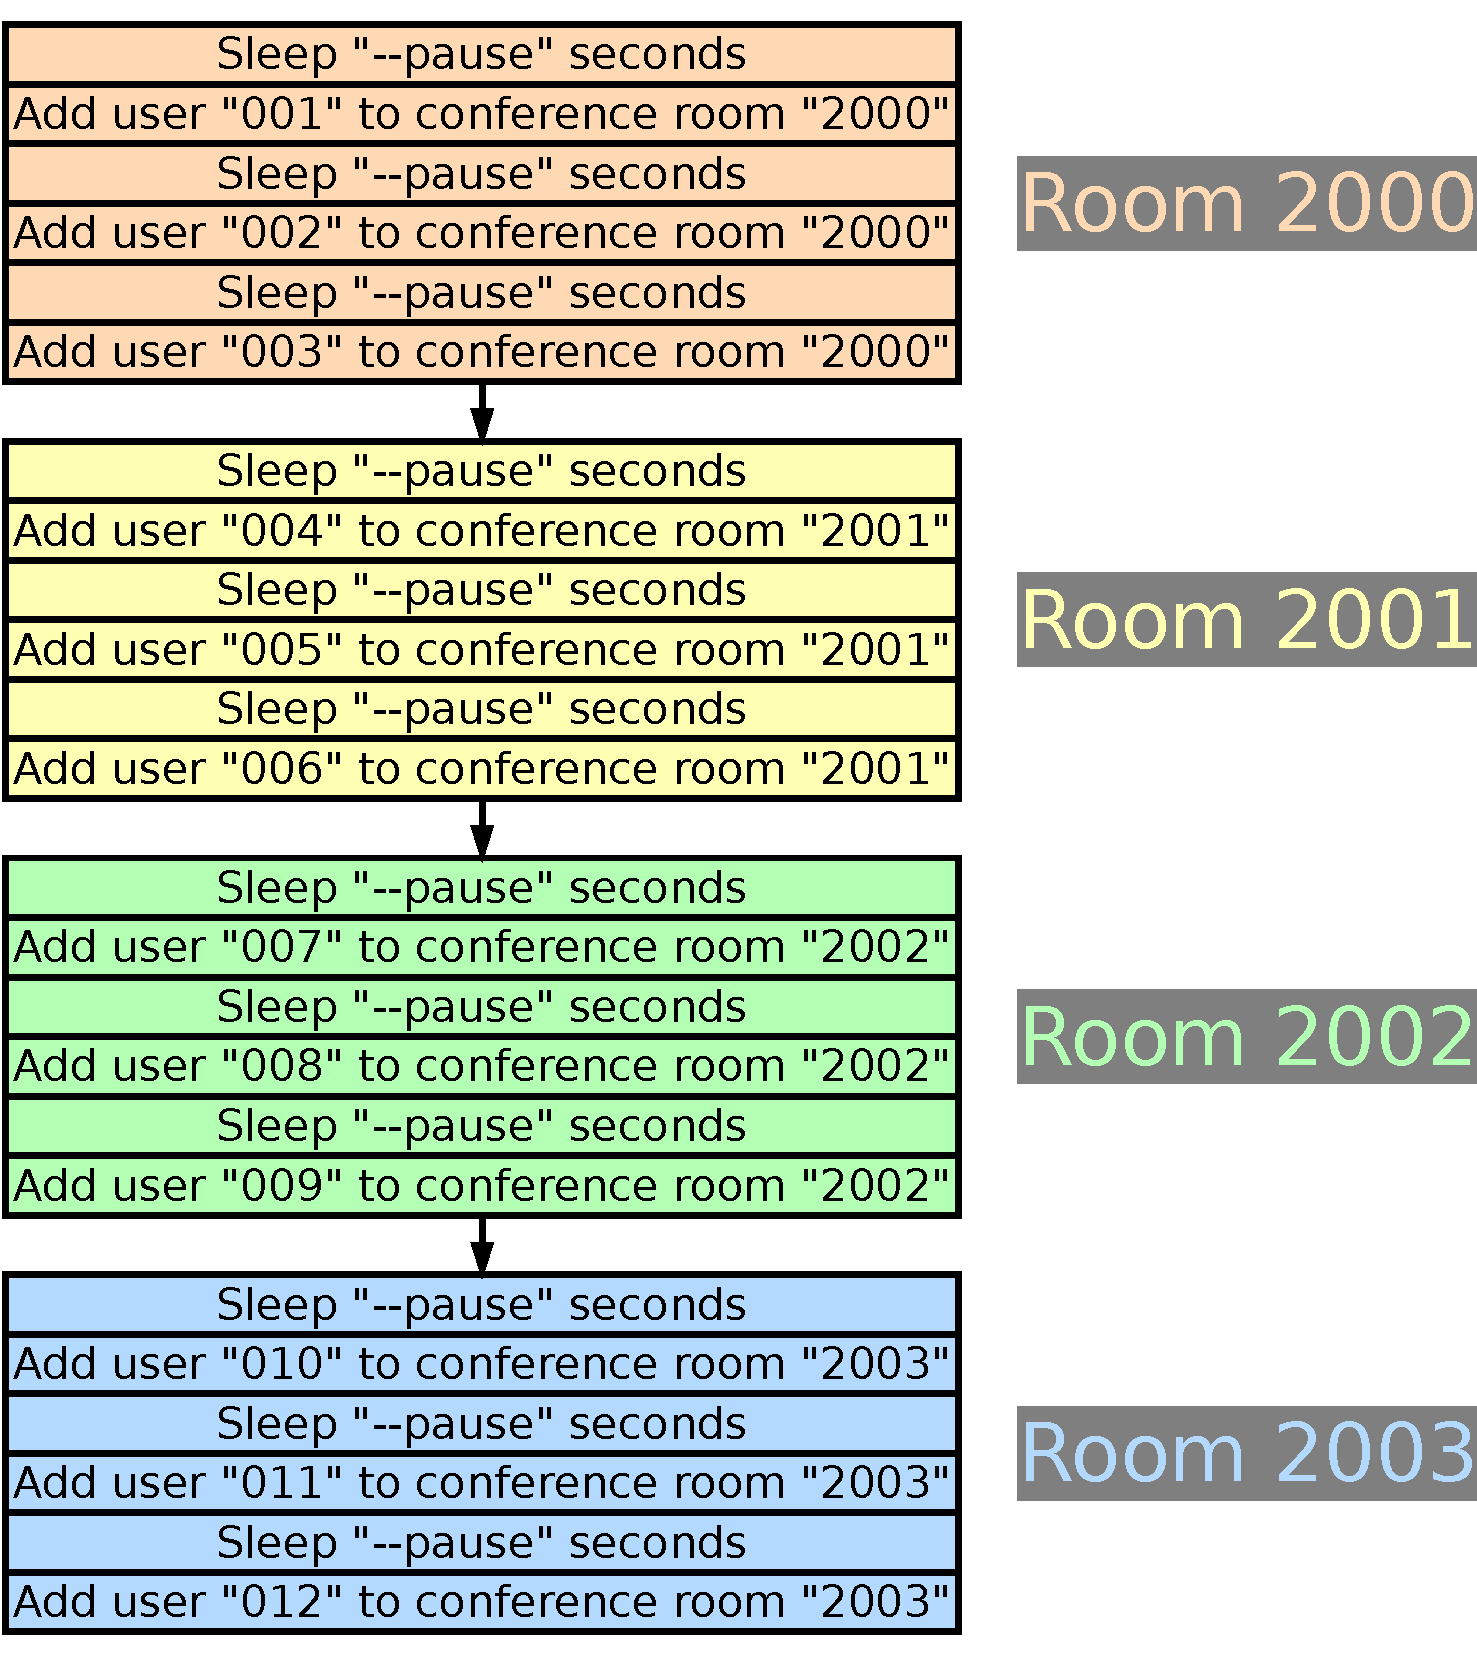
\includegraphics [width=8cm] {conf-rooms-test-2}
\caption{Conference rooms test example}
\end{figure}

This is implemented by using the sipp functionalities \texttt{call rates} (parameter -r)  and \texttt{rate period} (parameter -rp):
\begin{lstlisting}[breaklines=true,label=code:conf-call-invite,caption={sipp command for starting conf call tests} ]
sipp -aa -r 1
    -i $local_ip
    -rp 60s 
    -inf 'Users_conf-rooms.csv'
    -m $current_users
    -p 5061
    -mp 6020
    -sf 'Invite.xml'
    $ask_ip 2>&1"
\end{lstlisting}

\texttt{-rp 60s} is the rate period in seconds; \texttt{-r 1 -rp 60s} means that 1 user is added
every 60 seconds. With this scenario, the following situation is simulated:

\begin{figure} [!ht]
\centering
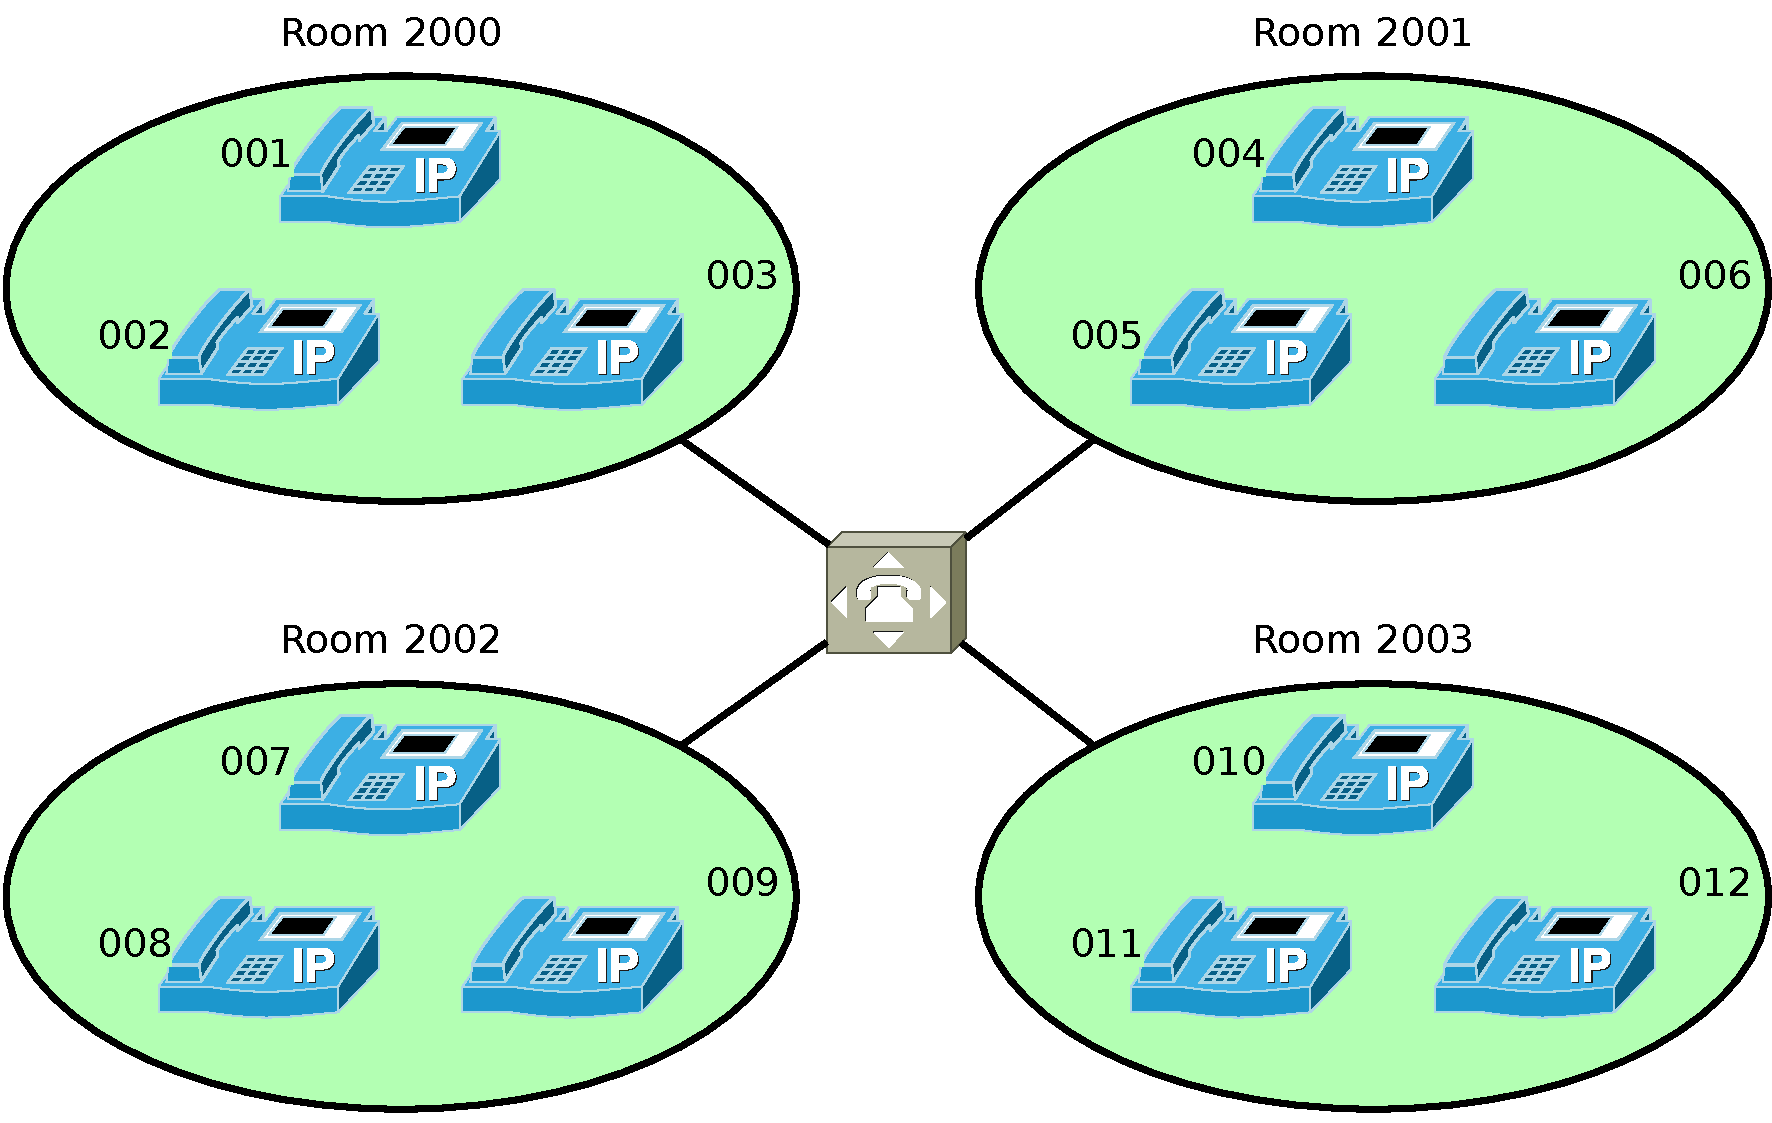
\includegraphics [width=10cm] {conf-rooms-test-3}
\caption {Conference rooms test illustration with 3 calls, 4 rooms}
\label {fig:conf-call-illustration}
\end{figure}

